\documentclass{article}
\usepackage{multicol}
\usepackage{graphicx}% Include figure files
\usepackage{dcolumn}% Align table columns on decimal point
\usepackage{bm}% bold math
\usepackage{hyperref}% add hypertext capabilities
\usepackage{booktabs}
\usepackage{listings}
\usepackage{mathtools}
\usepackage{amsmath}
\renewcommand{\abstractname}{\vspace{-\baselineskip}}
\bibliographystyle{plain}
\usepackage[utf8]{inputenc}
\usepackage{verbatim} %for å inkludere filer med tegn LaTeX ikke liker
\usepackage{mathpazo}
\usepackage{float}
\usepackage{algpseudocode}
\newcommand\numberthis{\addtocounter{equation}{1}\tag{\theequation}}
\usepackage[left=20mm,right=20mm,top=33.95mm,bottom=33.95mm]{geometry} 
% Justerer bredden på columns.
\setlength{\columnsep}{1cm}

\begin{document}

\title{Simulating the Solar System}
\author{Sebastian Amundsen, Marcus Berget and Andreas Wetzel}

\maketitle

\begin{abstract}
In this project we have created a model for simulating the solar system, with the final goal of testing whether it can successfully produce the expected values of the perihelion precession of Mercury around the sun. We started with simulating the simple Earth-Sun system, which gave a good testing ground for comparing the velocity Verlet method against the forward Euler method. We also tested whether the model was consistent with known Newtonian laws. We found the velocity Verlet method superior due to better stability and conservation of energy. We extended the model successfully by first including Jupiter, and then the rest of the planets. The model is consistent with Kepler's second law and conservation of energy, but unsuccessful in obtaining the correct value of the perihelion precession of Mercury. Our model predicts it would be -2.8575 arcseconds per century,  when it should be 42.9799 arcseconds per century. We couldn't figure out the reason for why our model misses that much.
\end{abstract}

\begin{multicols}{2}

\section{Introduction}

Though simulating a solar system is interesting and fun enough on it's own, it is naturally also quite useful for the study of astrodynamics. In addition, being able to simulate a solar system provides a good set of tools applicable to many other scientific areas. These tools include having a good understanding of different numerical integration methods, and being able to write a structured and fast code. In this project we wish to explore a model of our own solar system, beginning with simulating the simple two-body system including the Earth and the Sun. We will use this system to compare two different methods of numerical integration, the forward Euler method and the velocity Verlet method. This simple system also makes a good testing ground for exploring whether our model is consistent with known physical laws such as energy conservation and Kepler's laws of planetary motion. We will also test the stability of the velocity Verlet method by including Jupiter and playing around with it's mass. From there we will include the rest of the planets in our solar system, showcasing whether our code is applicable for many-body problems. At last, we will add a relativistic correction term to the force of gravity and check if we then observe the expected values of the perihelion precession of mercury.

\section{Method}
\subsection{Forward Euler}
The forward Euler method is an algorithm to estimate the solution of a differential equation. The Forward Euler method  finds the next positions $\mathbf{r}_{i+1}$ by using the position we are at $\mathbf{r}_{n}$, a small time step $dt$ and the derivative of its position. The forward Euler algorithm updates the position before the velocity, causing the energy to not be conserved.  
The forward Euler algorithm goes as follows:
\begin{verbatim}
v[0] = v0   # Boundary conditions
r[0] = r0   # Boundary conditions

for (n = 1; n < N-1; n++) {
V[n+1] = v[n] + a[n] * dt;
r[n+1] = r[n] + v[n] * dt;
t[n+1] = t[n] + dt;

}
\end{verbatim}
Where we count 4 FLOPs for every time step. The number of total FLOPS is $4N$, since we are looping over a time period N. It is also important to notice that the forward Euler method does not conserve energy. This is due to the position being updated before the velocity.  \\
For more details see C.1 Appendix.
\\
\subsection{Verlet integration}
The Velocity Verlet method is based on the kinematic equations for a moving object, which in our case is the planets orbiting around the sun. For the Velocity Verlet algorithm the velocity will be updated before the position, which leads to conservation of energy.\\   
The algorithm goes as follows:
\begin{verbatim}
v[0] = v0;   # Boundary conditions
r[0] = r0;   # Boundary conditions

for (i = 1; i < n-1; n++) {
v[n+1] = v[n] + (a[n+1]-a[n]) * dt / 2
r[n+1] = r[n] + v[n] * dt + a[n] * dt * dt / 2;
}

\end{verbatim}
where we count 10 FLOPs for every time step. 
For more details see C.2 Appendix.

\subsection{Program flow}

We will here discuss the program flow of the code we have used to model the solar system. All code can be found at the GitHub repository \\
\url{https://github.com/Sebamun/FYS3150_Projekter/tree/master/Project3}  \\ The code is mostly based on two classes, a planet class and a solver class. Initializing the planet class creates an instance which contains all the relevant information about a celestial object. When the desired celestial objects are initialized, they can then be added to an instance of the solver class. The solver class contains many different functions, mostly aimed toward aiding the velocity Verlet or Euler function. These two functions are based on using their respective algorithms to print out the relevant information of each time step to output-files. The output files can then be read by python-programs which analyze/plot the data.

\subsection{Comparison of the algorithms}
The timing and counting of number of FLOPS of the algorithms is done by writing two separate programs with the sole purpose of doing only this. Comparing the stability of the algorithms is done by plotting the earth-sun system for different time-steps, with the Sun as the center of mass. For the case of a circular orbit we expect that both the potential and kinetic energies are constant and conserved. This is naturally also something we check that the algorithms uphold. We test both algorithms with integration points $N=10^5$, $N=10^6$ and $N=10^7$. This will tell us how fast our two integration methods are. We will also test the accuracy of each algorithm with integration points $N=1000$, $N=5000$ and $N=10000$. This will give us a clue for which algorithm that is best to use in our specific case. 

\subsection{Earth-Sun system}

We have used the Earth-Sun system to compare the two algorithms, but we will now proceed by ditching the forward Euler method, using only the velocity Verlet method instead. Kepler's second law of planetary motion states that the imaginary line joining a planet and the sun sweeps equal areas of space during equal time intervals as the planet orbits \cite{94}. As shown in  appendix B.2, this is equivalent to conservation of angular momentum. We know that the gravitational force is an inverse square force. We wish to know what would occur if we changed this force to a higher order inverse force. This is explained in B.3 Appendix.

\subsection{Many-body system}

Before we include all the planets of the solar system, we start by including only Jupiter. But instead of using our own manufactured initial conditions, we extract the initial conditions from the NASA website \url{https://ssd.jpl.nasa.gov/horizons.cgi#top}. We write the initial conditions to a text file, before we convert the velocities to $\text{AU/Y}$. We also have to take into account, that the velocities extracted from NASA is relative to the center of mass. We therefore have to subtract the velocity of the center of mass to all the velocities. The velocity of the center of mass of the system is found by:
\begin{align}
v_{cm} = \frac{\sum v_i m_i}{M}
\end{align}
where $M$ is the total mass of all the objects in the system, and $v_i$ and $m_i$ are the respective velocities and masses of the objects. We will test our three body problem with different masses for Jupiter. We want to see how this impacts the orbit of the objects. The mass is increased by a factor of ten and a factor of 1000 for Jupiter. 

Finally we are going to use the Verlet algorithm to simulate all the planets in the solar-system. We study a time period of 170 years. 

\subsection{Perihelion precession of mercury}

Just like all the other planets in orbit around the sun, mercury's orbit has an perihelion precession. However, unlike the other planets, mercury's precession can't be explained only by the gravitional tug from other solar bodies. The observed value of the perihelion precession due to relativistic effects is 42.9799 arcseconds per century \cite{97}. The deviation can be explained by general relativity by adding a correction to the Newtonian gravitational force, so that the force becomes
\begin{equation}
\mathbf{F}=-G\frac{M_{\odot}M_{Mercury}}{r^2}\Bigg[1+\Bigg(\frac{3l^2}{r^2c^2}\bigg)\bigg]\frac{\mathbf{r}}{r} \label{eq:relcor}
\end{equation}
where $M_\odot\ $ is the mass of the Sun, $M_{Mercury}$ is the mass of Mercury, $r$ is the distance between Mercury and the Sun, $l = |\vec{r} \times \vec{v}|$ is the magnitude of Mercury’s orbital angular momentum per unit mass, and $c$ is the speed of light in vacuum. We want to see if our code produces the same observations, so we start by initializing the system by setting the Sun in the center with Mercury in it's perihelion postition. The distance from Mercury to the Sun at perihelion postition is 0.3075 AU, with a speed of 12.44 AU/yr. We then set the simulation time to 100 years. Since we only want to observe the change in precession due to the correction in the gravitational force, we only simulate the Sun and Mercury. Since 43 arc seconds is a very small change in precession, we use as many integration points as possible. To avoid creating too large text files with information about every timestep, we set up the code such that if we use more than $10^7$ integration points, the code only prints out the final position, and velocity to the text file. We then use those positions and velocities as initial conditions for an additional run where the simulation time is about 0.3 years (a little more than a full orbit of mercury around the sun). We then find which time step the minimum distance between the Sun and Mercury took place. We then use this time step to find how much the y-value of the perihelion position has changed. Finally, we can use this value to find the perihelion precession using
\begin{equation}
\tan(\theta_P) = \frac{y_P}{x_P}
\end{equation}

\section{Results}

Figures are given in A appendix. 

\subsection{Comparison of the algorithms}

\begin{table}[H]
\begin{center}
\caption{The speed of the different algorithms.}
\begin{tabular}{  |c|c|c|c|c|c| } \hline
Algorithm&$N=10^5$&$N=10^6$&$N=10^7$ \\ \hline
Euler&0.30419 s&2.89849 s&33.3088 s\\ \hline
Verlet&0.37503 s&3.16336 s &38.3016 s \\ \hline
\end{tabular}
\label{tab:Algo_N}
\end{center}
\end{table}

The time it took to run the different algorithms is given in Table \ref{tab:Algo_N}. The plots for the different algorithms with different integration points is given in Figure \ref{fig:Acc}.

\subsection{Earth -Sun system}

We can see the behavior for the Sun-Earth system with different initial velocities in Figure \ref{fig:esc}. We see that by using the analytical value for the escape velocity of $v_{esc}=2 \sqrt{2} \pi $ the Earth escapes the sun's gravitational field. By trial and error, we found that the highest velocity we could initialize the earth with was $\sqrt{7.81} \pi$ (with a simulation time of 100 yrs and $5\cdot 10^6$). 

We can see the different planetary motion of earth as we adjust $\beta$ in Figure \ref{fig:Force_beta}.

The angular momentum is given in Figure \ref{fig:angmon} for the Velocity Verlet algorithm. 

The energy for the Velocity Verlet is given in Figure \ref{fig:Energy}.

\subsection{Many-body system}

We can see the different orbits of the three body problem with varying masses for Jupiter in Figure \ref{fig:Jup_mass}. We solved the many body problem with 8 planets and the sun and the plot is given in Figure \ref{fig:Solar}. 

\subsection{Perihelion precession of Mercury}
\begin{table}[H]
	\caption{Table of the computed perihelion precession, with and without the general relativistic correction, and the difference between them. The number of integration points used in this simulation was $10^8$.}
	\label{table:peri}
	\begin{tabular}{l|l}
		\hline
		Perihelion precession angle \\ w/  GR correction  & -619.0085 arcseconds \\ \hline
		Perihelion precession angle \\ w/o GR correction & -616.1510 arcseconds   \\ \hline
		$\Delta \theta_p$& -2.8575 arcseconds   \\ \hline
	\end{tabular}
\end{table}

\section{Discussion}

\subsection{Program flow}
As mentioned above, the code is set up such that it creates text files for each simulation. One issue with this specific setup, is that when a simulation is run with the same amount of bodies as a preexisting one, the old text file will be overwritten. This could easily been fixed by making the function which prints information depend on more parameters, so that the name of the text file could be personalized even further. 

\subsection{Comparison of the algorithms}

We can see from Table \ref{tab:Algo_N} that the Verlet method is slower than the Euler method. This is to be expected given the number of FLOPS in the Verlet method compared to the Euler method. In Figure \ref{fig:Acc} we can see that the Verlet method is more precise at lower integration points than Euler. When we increase the number of integration points, the orbits given the two methods become more equal. Since the Euler method is quicker, there is an argument to use Euler at higher integration points. However, it is important to note that over longer time periods the Euler method becomes less viable. This is due to the fact that the Euler method dosen't conserve energy. 

\subsection{Testing forms of the force}

As we increase $\beta$ in equation \ref{eq:F_b} we see that the orbit becomes more unstable (Figure \ref{fig:Force_beta} ). An increased $\beta$ leads to a smaller gravitational force, this could be the reason for the unstable orbits. We keep the initial distance form the sun and decrease the force that works on the planet, which would make it easier for the planet to escape. When this force is lower than a certain threshold we will lose our planet from orbit. In our case this limit was at $\beta=2.99$.

\subsection{Escape velocity}

If we increase the initial velocity we see that the orbit of the earth changes from a circular orbit to an elliptical one. When the elliptical orbit increases the position between the two object will also increase. Hence, the force of gravity will decrease. And when the initial velocity of the planet make it to the escape velocity it will tear loose from the gravitational field.

\subsection{Many-body system}

When we increase the mass of Jupiter we will see that the force that is exerted on the sun and earth increases. This leads to a more unstable orbit for all objects. For the mass of Jupiter $\times 10$ we stil have an orbit around the sun, but it is somewhat more unstable. When we increase the mass of Jupiter by 1000 we lose our elliptical orbits. We can see the earth being "slinged" out of the system. This is due to the drastically increased force from Jupiter. When the earth gets close to the two other objects, the forces on the earth accumulate and gives the planet an acceleration which is big enough to escape the gravitational pull from the sun (Figure \ref{fig:Jup_mass}). 

We wanted to have a full rotation around the sun for all the planets. The outer most planet Neptune reached a full orbit after a period of 170 years, which became the time we run our simulation with. In this time span the inner planets managed to preform multiple orbits around the sun. The later orbits changed relative to their original orbit, which is to be expected given that the sun and planets move over time. That is why the lines become thicker towards the center of the plot (Figure \ref{fig:Solar}. 

\subsection{Angular momentum and energy}

The analytical part shows that the angular momentum is conserved. But when we look at Figure \ref{fig:angmon} it looks as if the angular momentum has not been conserved. This is because the algorithm fails to preserve angular momentum exactly. There will also be numerical errors, such as small deviations in the calculation. The change in angular momentum between each peak is really small, when taking into account the amount of time we run the simulation for. We can therefore say that the angular momentum more or less is conserved. 

We see from Figure \ref{fig:Energy} that the total energy is conserved for the Velocity Verlet algorithm. The energy has some fluctuations, but oscillates around the same constant energy level.

\subsection{Perihelion precession of mercury}
As we can see from table (\ref{table:peri}), we get that Mercury's precession without the relativistic correction is about -616 arcseconds per century, when we expect that it would be 0 arcseconds per century. There is obviously something in the code that goes wrong, and unfortunately we can't find what is the cause. The initial thought is that we're not using enough integration points, and it would be interesting to see if we could get a more accurate result by increasing the integration points even further. However, we do not believe this is the main cause of the inaccurate result.  We believe that there might be a bug in our code, or a systemic fault in the velocity Verlet function, but we're unsure of precisely what it could be. Another interesting observation is that the difference between the precession angles, with and without the relativistic correction is only about -2.86 arcseconds, when we would expect it to be around 43 arcseconds.  

\section{Concluding remarks}
Considering the minimal difference in time spent by the two algorithms, and the fact that the velocity Verlet method is both more stable and conserves energy, we find the velocity Verlet method to be superior compared to the forward Euler method for simulating a solar system. We can also conclude that our model using the velocity Verlet method is consistent with what we would expect from Kepler's second law, and conservation of energy. In addition, the model doesn't seem to have any issues with adding more planets. Unfortunately,  when adding the relativistic correction term we don't obtain the theoretical/observed values for the perihelion precession of Mercury.

\end{multicols}

\clearpage
\appendix \section{Appendix} % Her kommer appendix.

\begin{figure}[H]
	\centering
	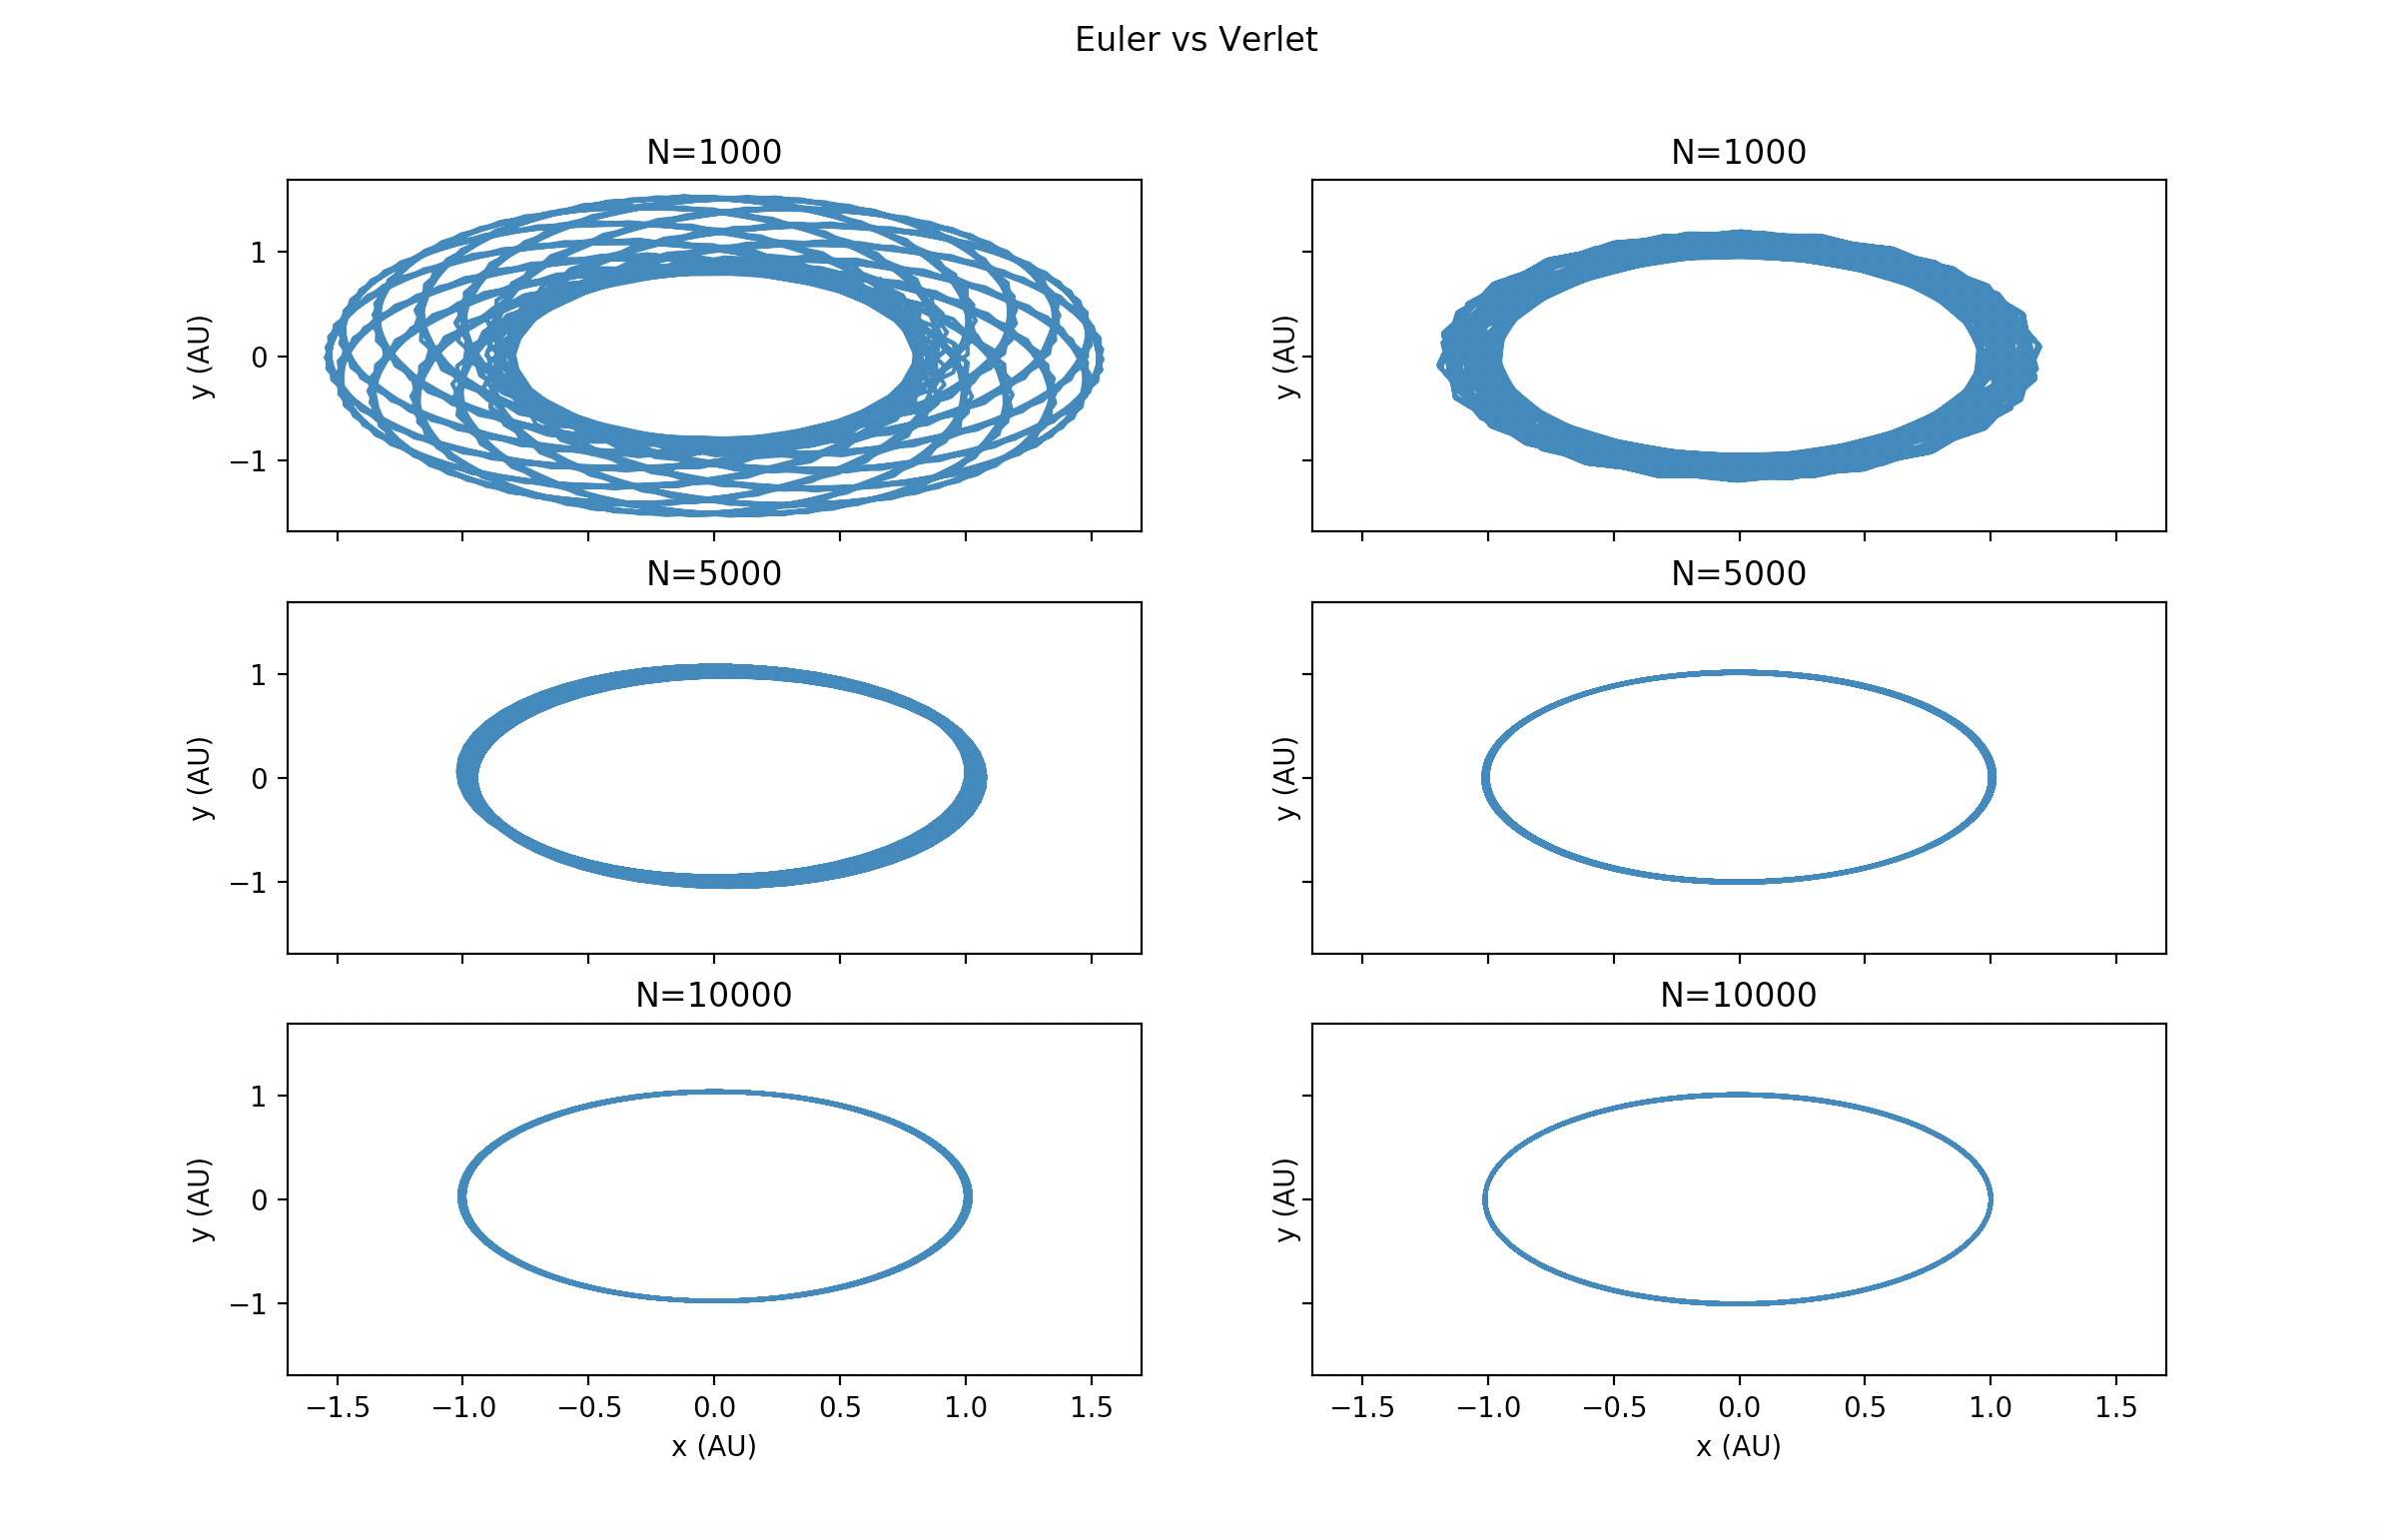
\includegraphics[width=120mm]{Acc}
	\caption{The accuracy of the different algorithms at different time steps.}
	\label{fig:Acc}
\end{figure}


\begin{figure}[H]
	\centering
	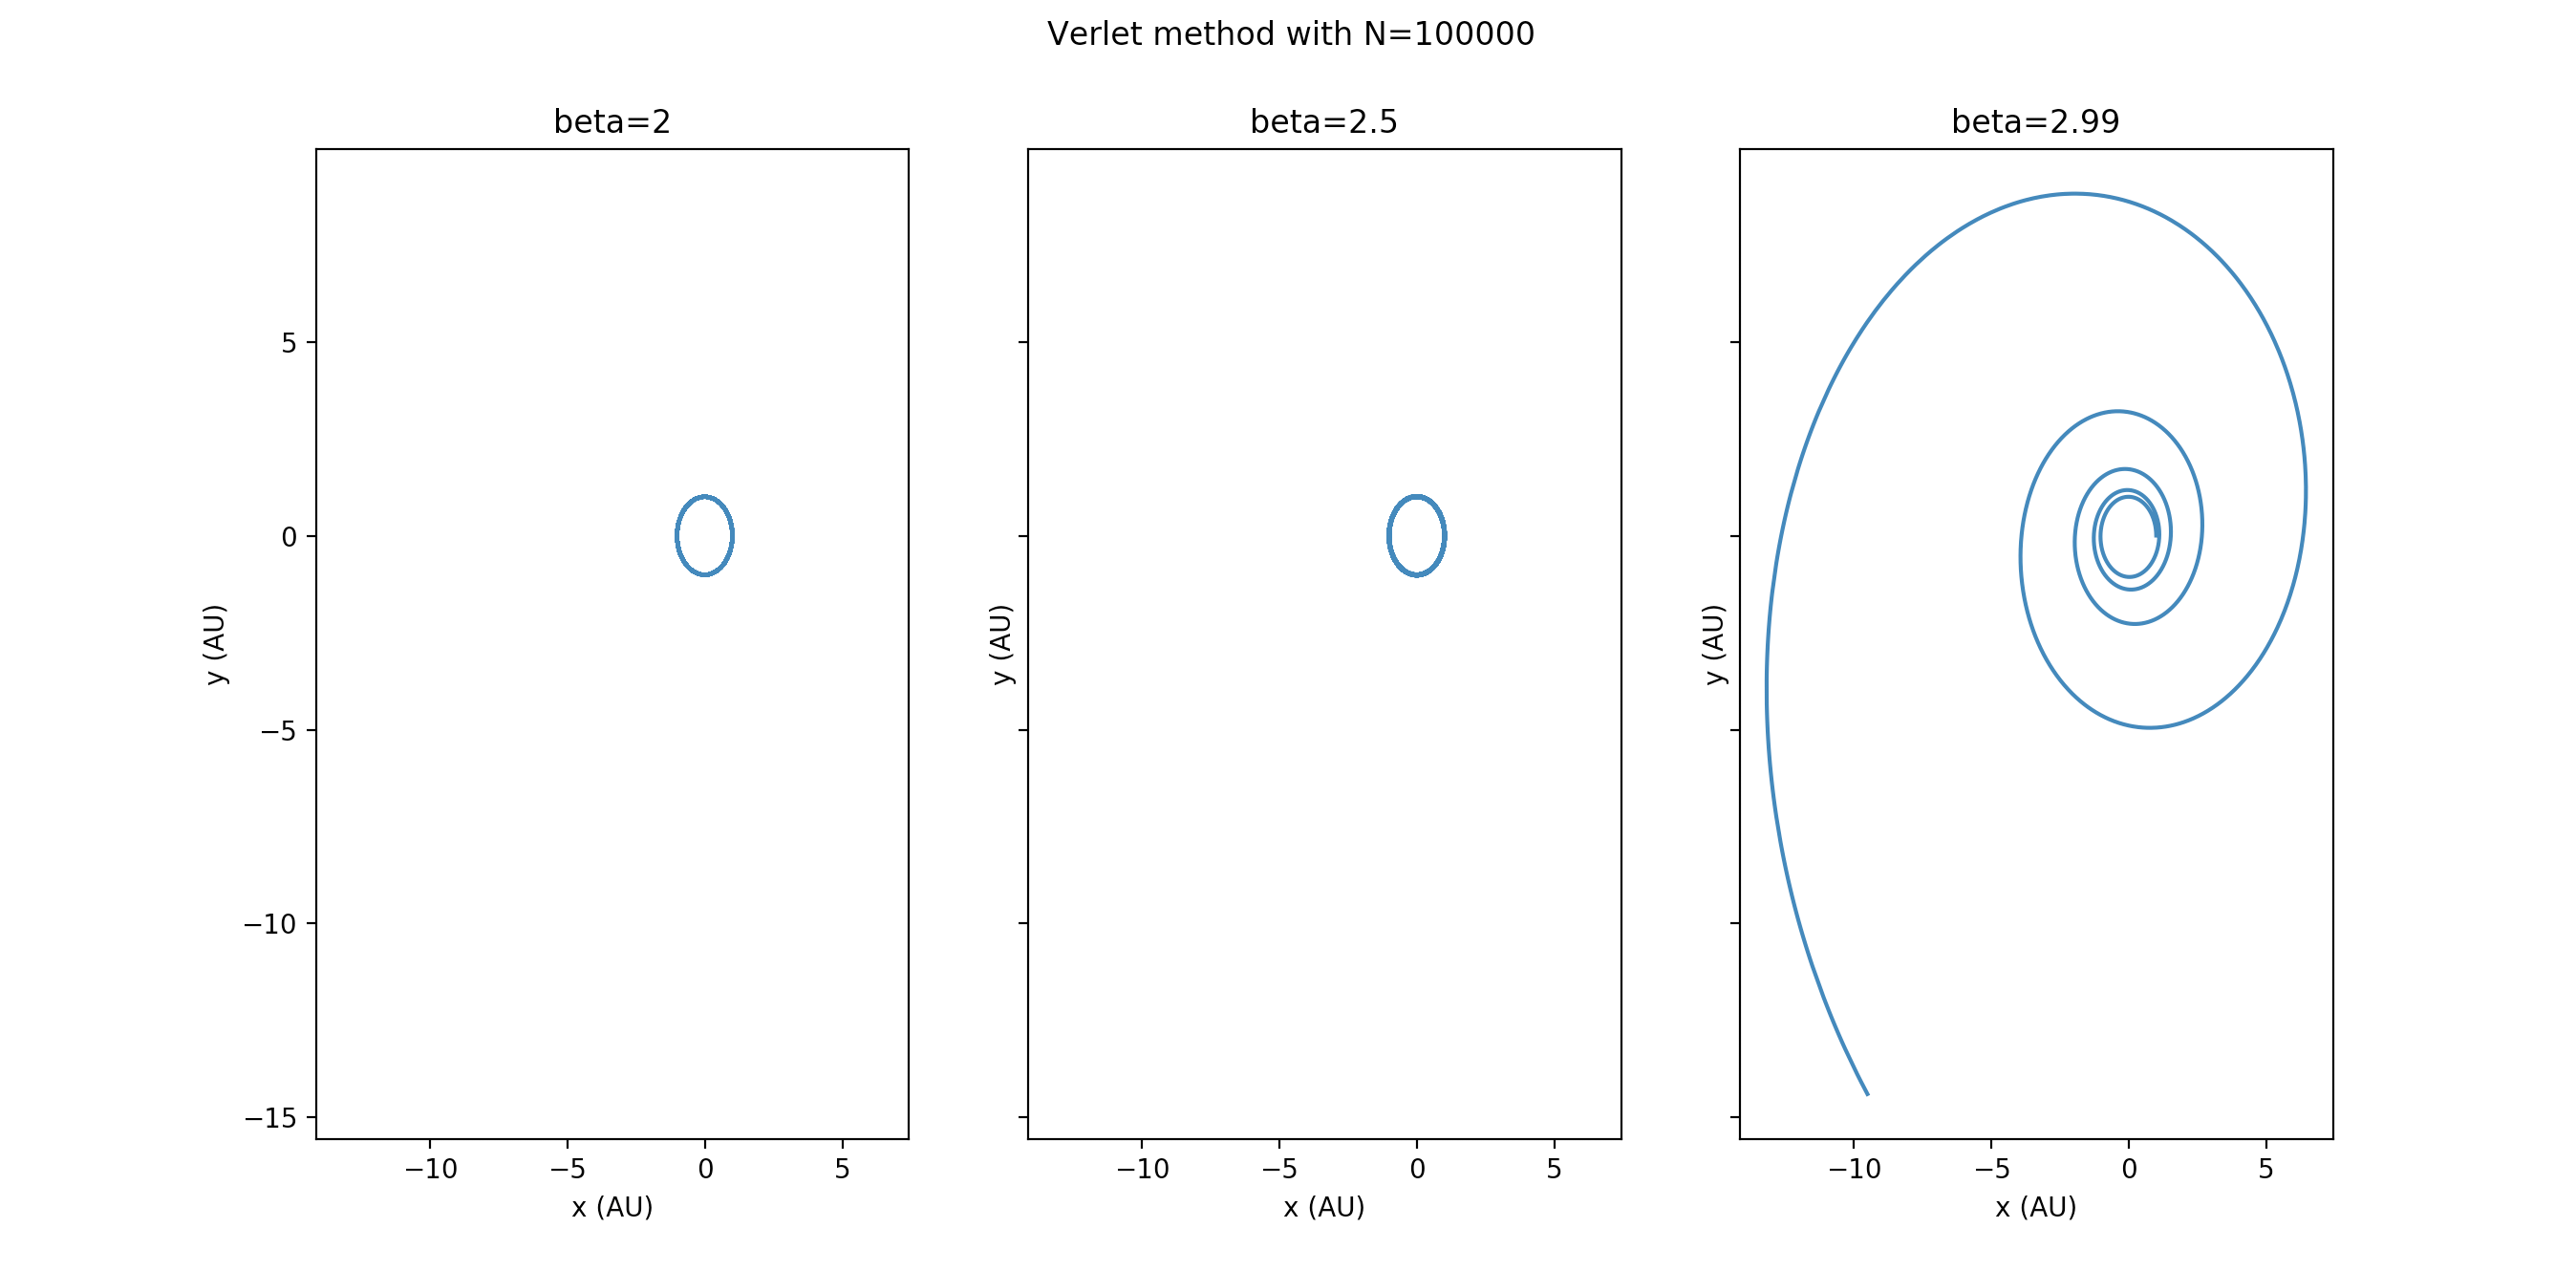
\includegraphics[width=120mm]{Force_beta}
	\caption{The planetary motion of earth at different $\beta$.}
	\label{fig:Force_beta}
\end{figure}


\begin{figure}[H]
	\centering
	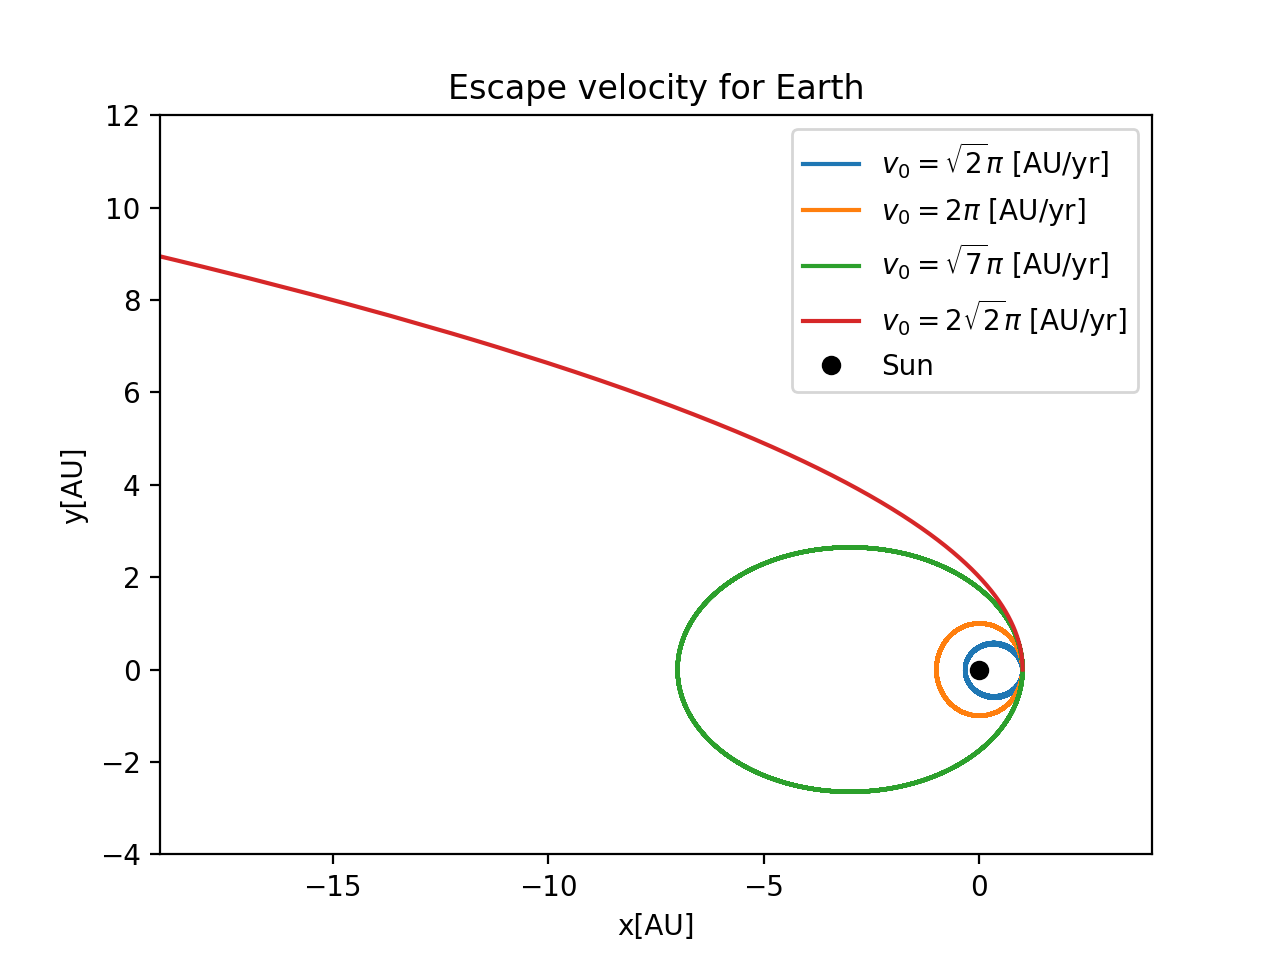
\includegraphics[width=120mm]{esc_vel_plot.png}
	\caption{Escape velocity for the Sun-Earth system for different initial velocity}
	\label{fig:esc}
\end{figure}

\begin{figure}[H]
	\centering
	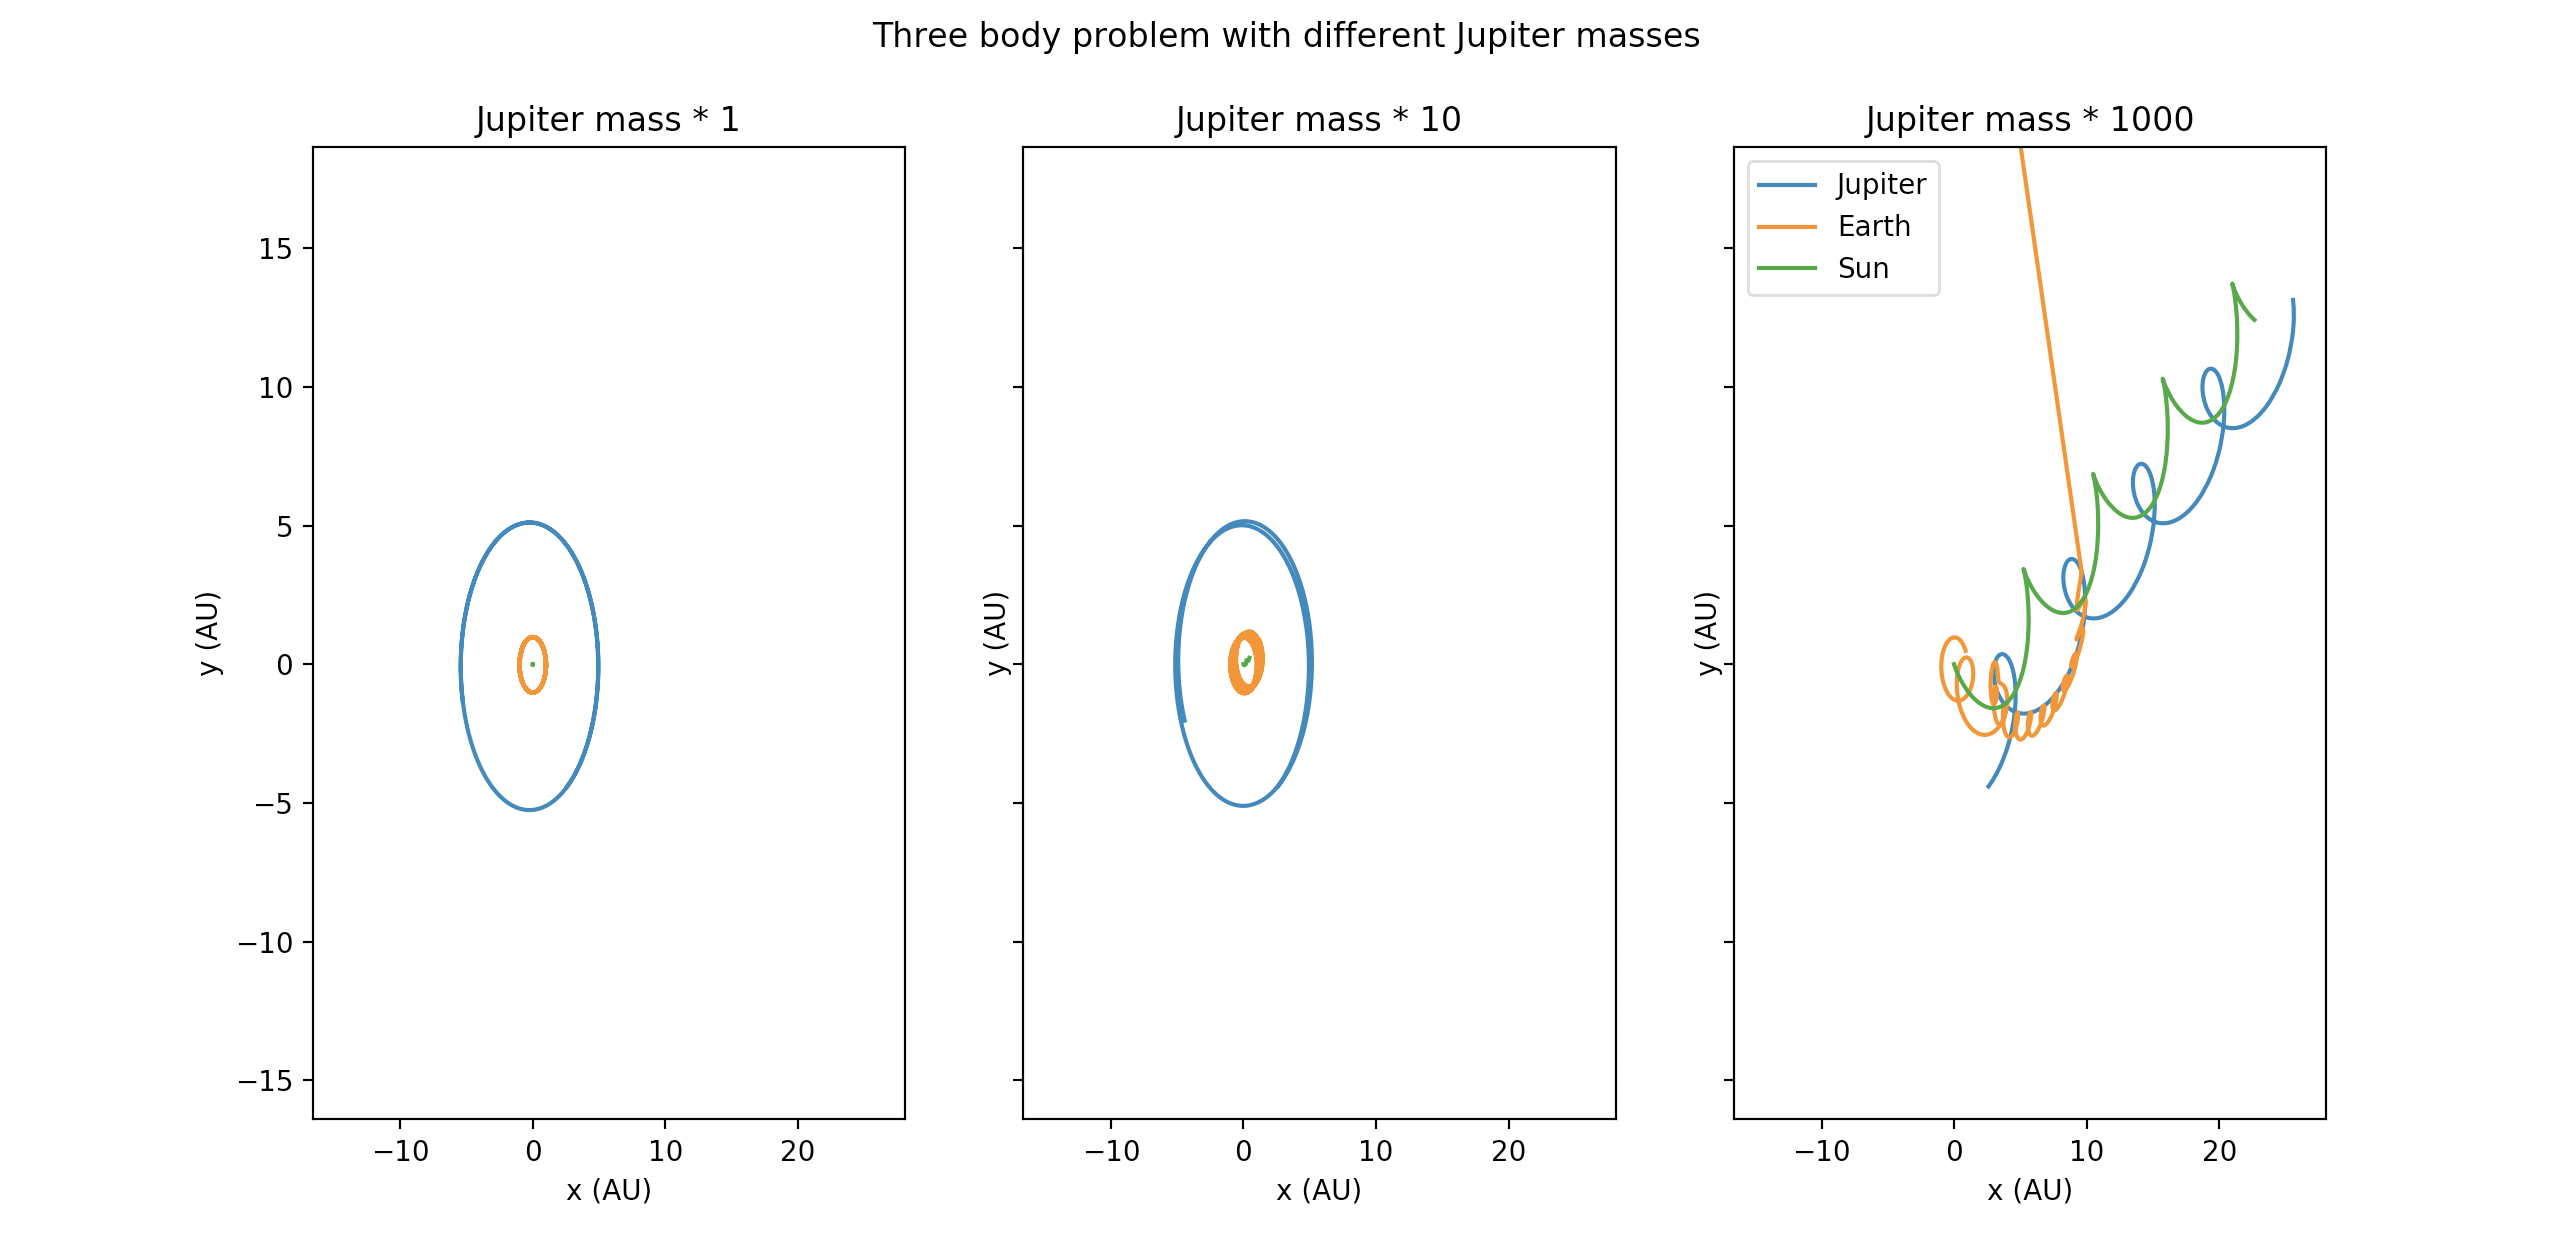
\includegraphics[width=120mm]{Jup_mass}
	\caption{Three body problem with varying Jupiter masses.}
	\label{fig:Jup_mass}
\end{figure}

\begin{figure}[H]
	\centering
	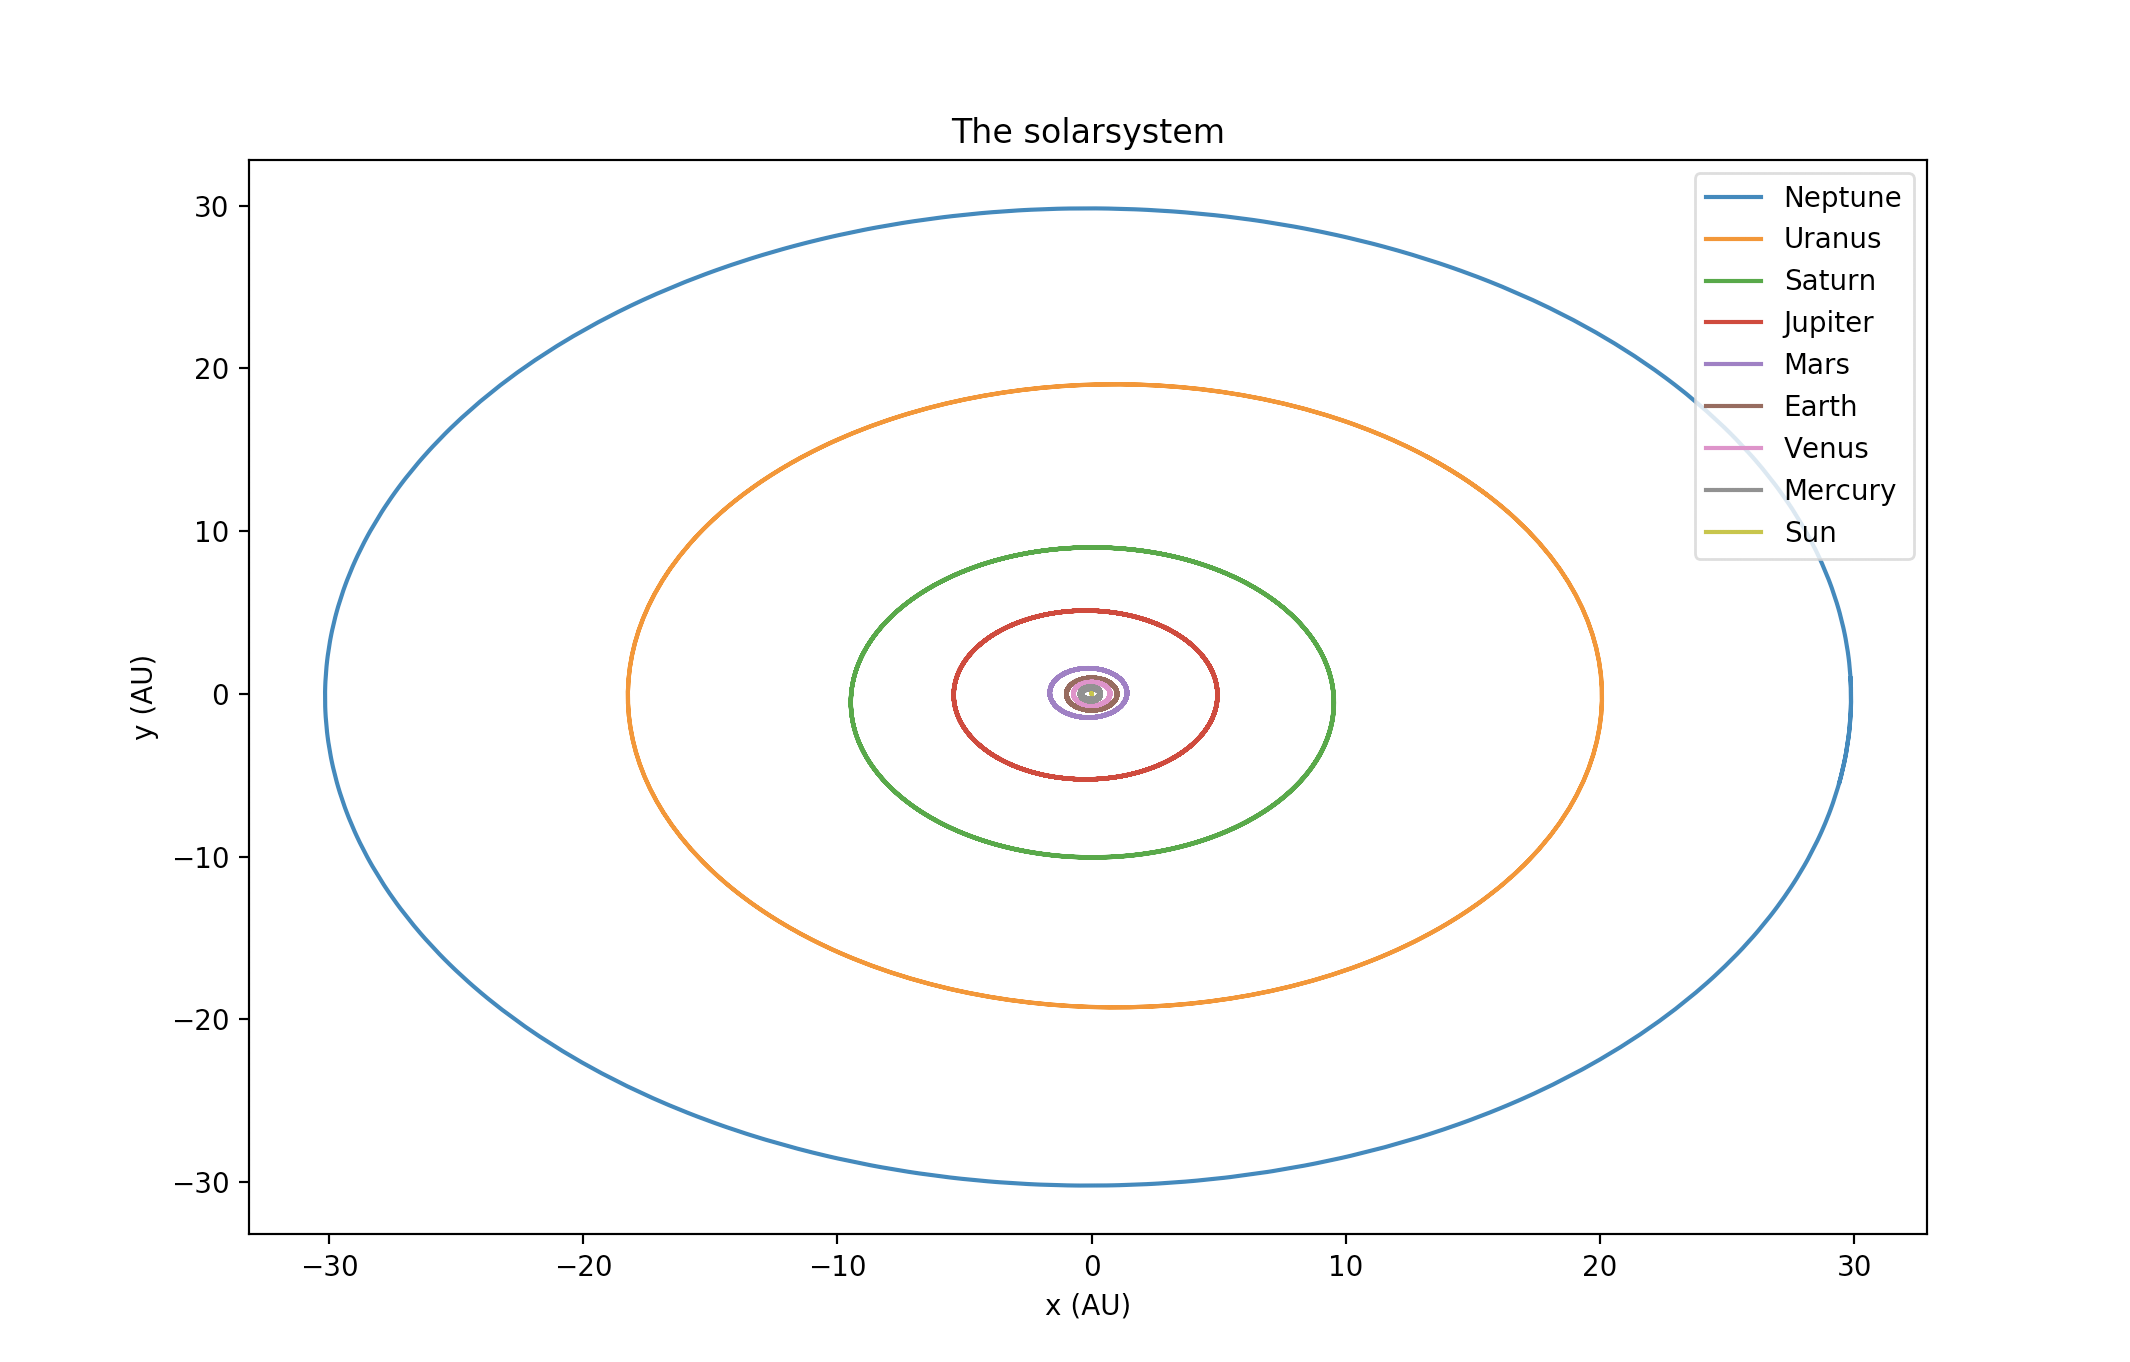
\includegraphics[width=120mm]{Solar}
	\caption{The solar system.}
	\label{fig:Solar}
\end{figure}

\begin{figure}[H]
	\centering
	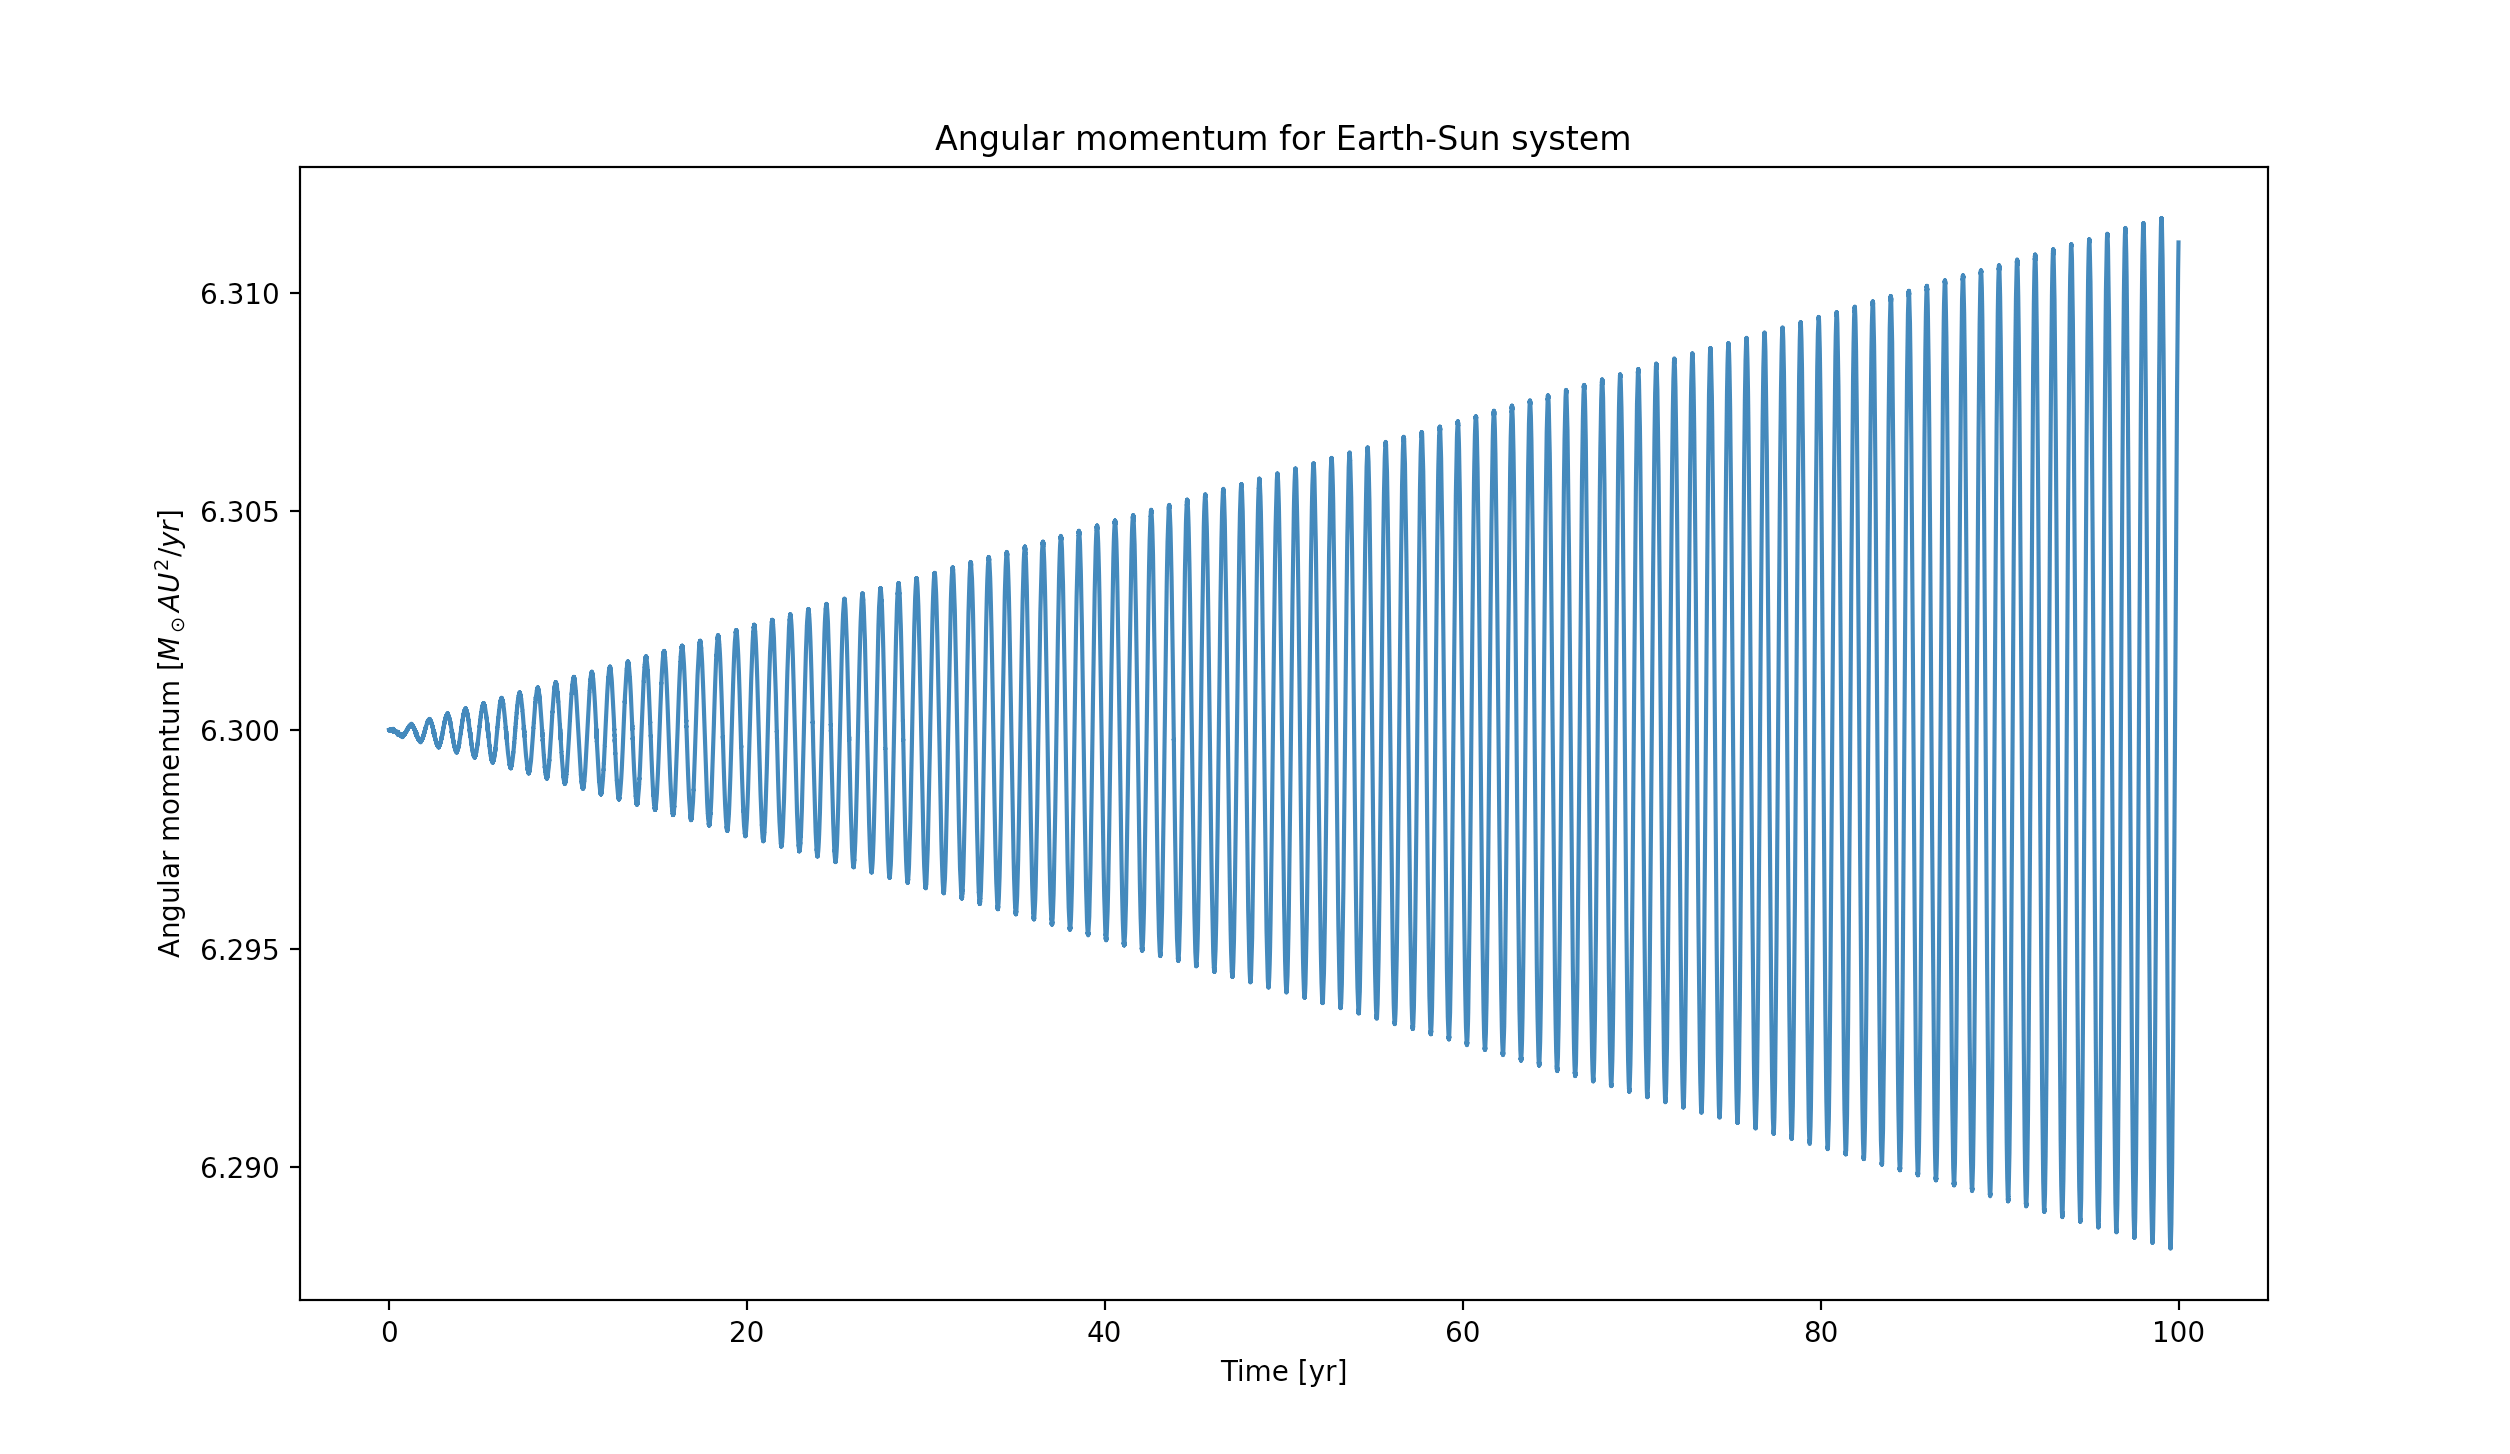
\includegraphics[width=120mm]{ang_mom_con.png}
	\caption{Conservation of angular momentum, Velocity Verlet algorithm  }
	\label{fig:angmon}
\end{figure}

\begin{figure}[H]
	\centering
	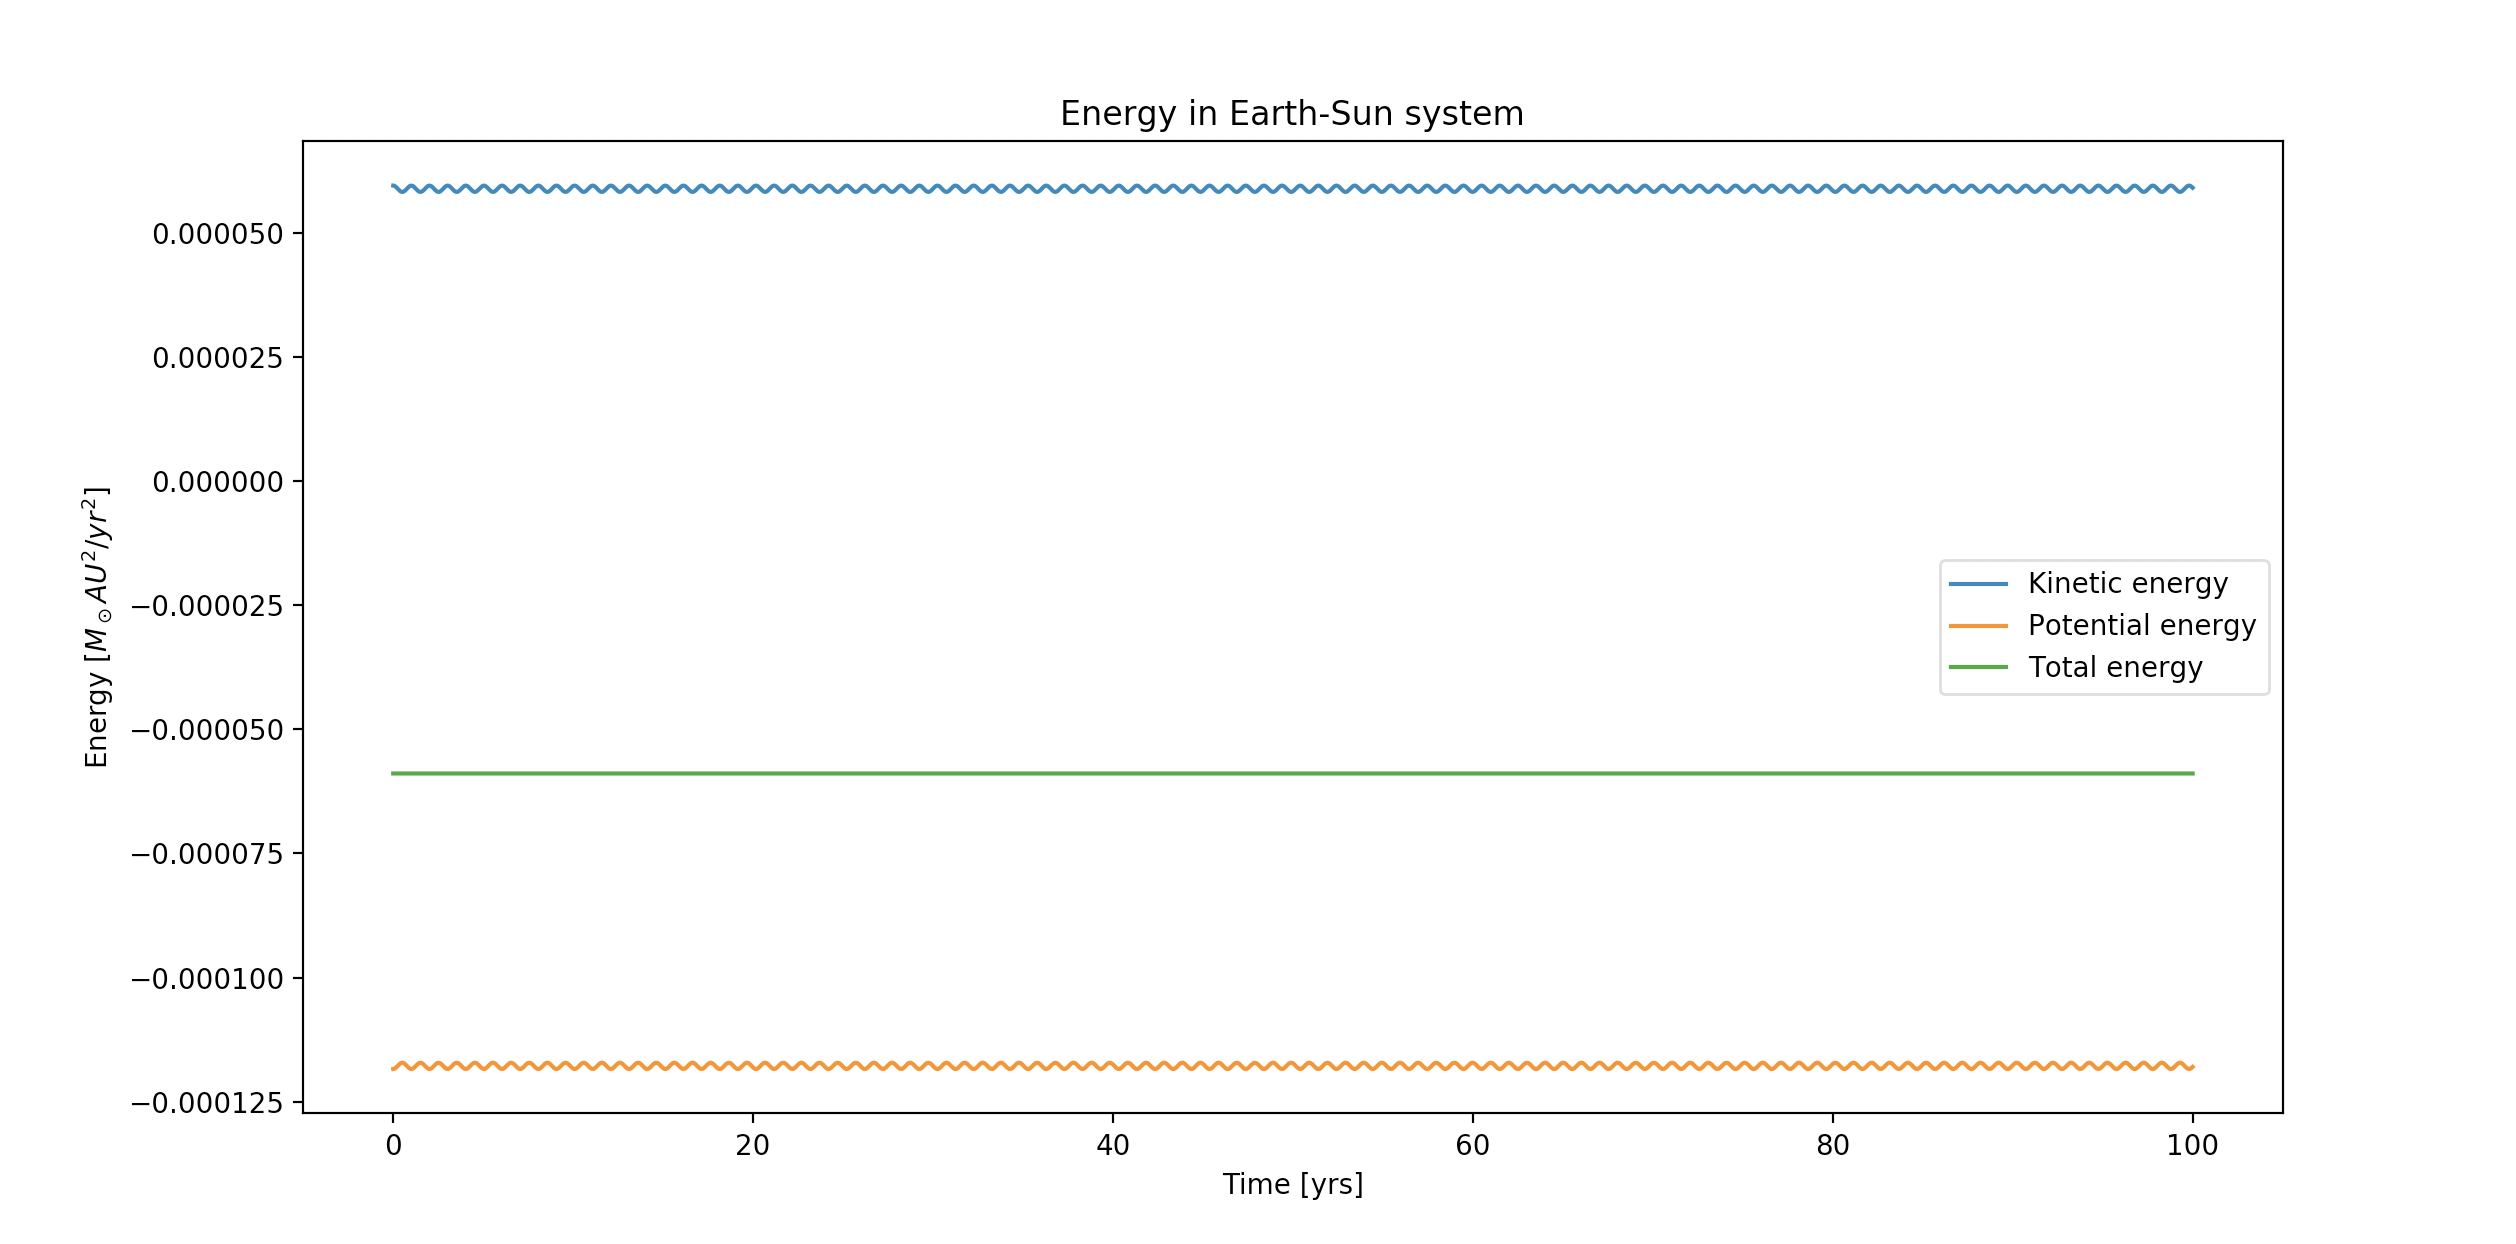
\includegraphics[width=120mm]{Energy}
	\caption{The kinetic and potential energy for Velocity Verlet.}
	\label{fig:Energy}
\end{figure}


\section{Appendix} % Her kommer appendix.
\subsection{The Earth-Sun system}
We assume that the earths orbit around the sun is circular. Circular motion and Newtons gravitational force gives us:
\begin{equation}
    F_G=G\frac{M_EM_{\odot}}{r^2}=\frac{M_Ev^2}{r}
    \label{eq:G}
\end{equation}
Where G is the gravitational constant, $M_\odot$ is the mass of the sun, $M_E$ is the mass of the earth, $r$ is the distance between the earth and the sun, and $v$ is the velocity of the moving object (earth). 

We want to show that the velocity $v$ can be written as:

\begin{align}
    v^2r=GM_{\odot}=4\pi^2\frac{AU^3}{yr^2}
    \label{eq:vr}
\end{align}

We can use the centripetal force to rewrite equation \ref{eq:G}, since we are assuming circular orbits:

\begin{align*}
    M_E\omega^2r=G\frac{M_EM_{\odot}}{r^2}
\end{align*}

Where $\omega^2$ is the angular velocity of the earth. Which is given by $\omega^2=2\pi / P$: 

\begin{align*}
    M_E\bigg(\frac{2\pi}{P}\bigg)^2r=G\frac{M_EM_{\odot}}{r^2}\\
\end{align*}

Where $P=1$ year is the period of earth's orbit around the sun. Now we can use Kepler's third law, which states that the square of an orbital period $P^2$ equals the semi-major axis as it orbits the sun cubed $a^3$. This gives us:

\begin{align*}
P^2=\frac{4\pi^2}{GM_\odot}a^3
\end{align*}
\begin{align}
    GM_\odot=4\pi^2\frac{AU^3}{yr^2}
    \label{eq:G_M}
\end{align}

\subsection{Conservation of angular momentum}

\begin{figure}[H]
	\centering
	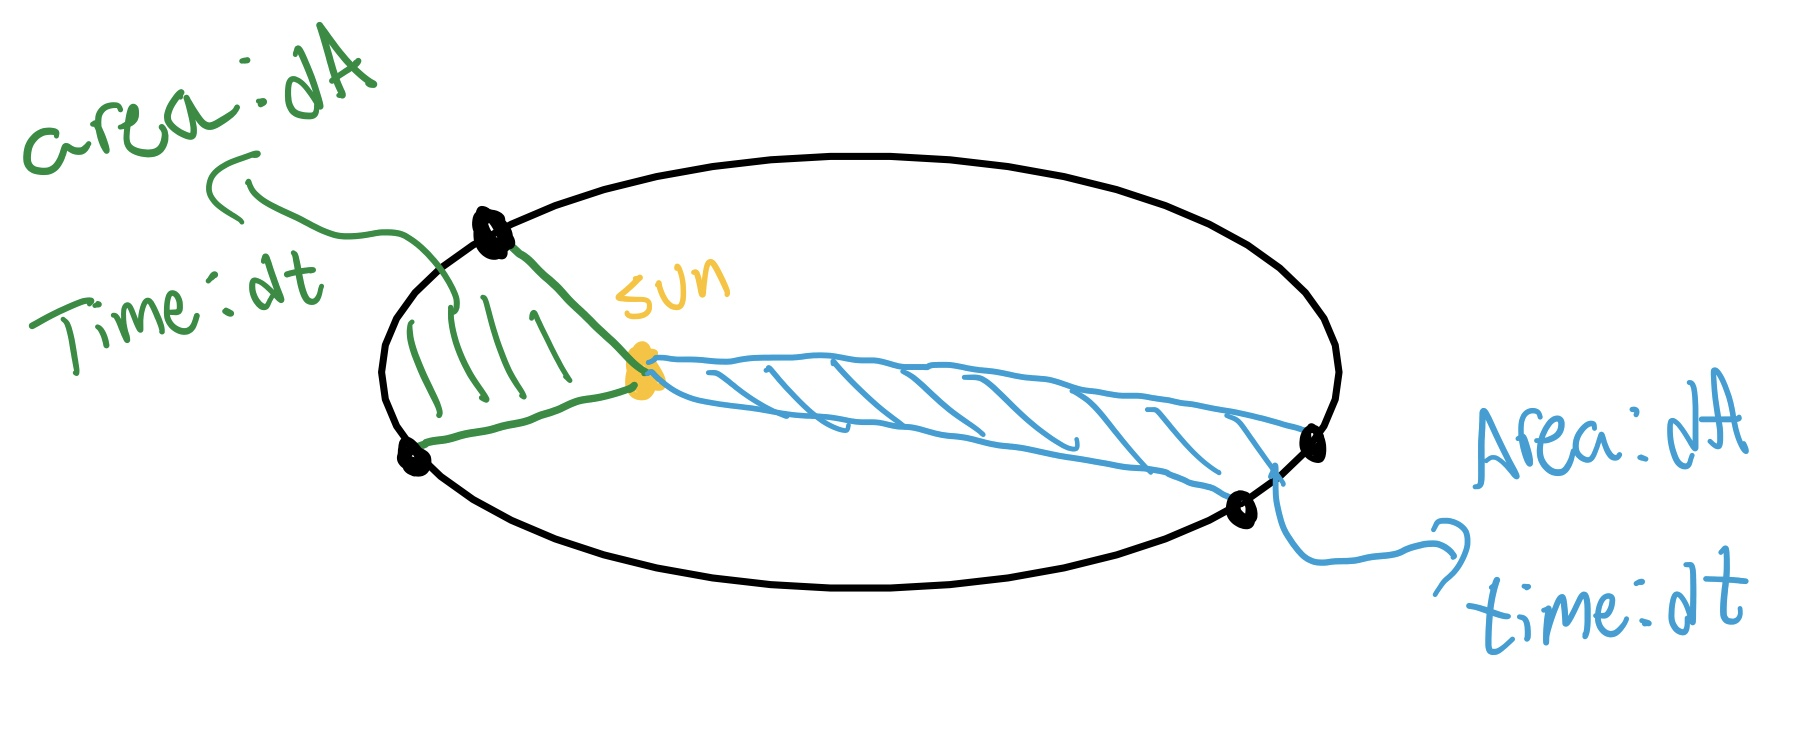
\includegraphics[width=80mm]{K2L.jpg}
	\caption{The area $dA$ is the same for the two time intervals.}
	\label{fig:Kep}
\end{figure}

The definition of Keplers law is that the area $A$, which is formed from a connecting line between a planet and the sun is always the same for a given time interval. This is illustrated in Figure \ref{fig:Kep}.

The best way to show that the angular momentum is conserved by using Keplers second law is to make a drawing:

\begin{figure}[H]
	\centering
	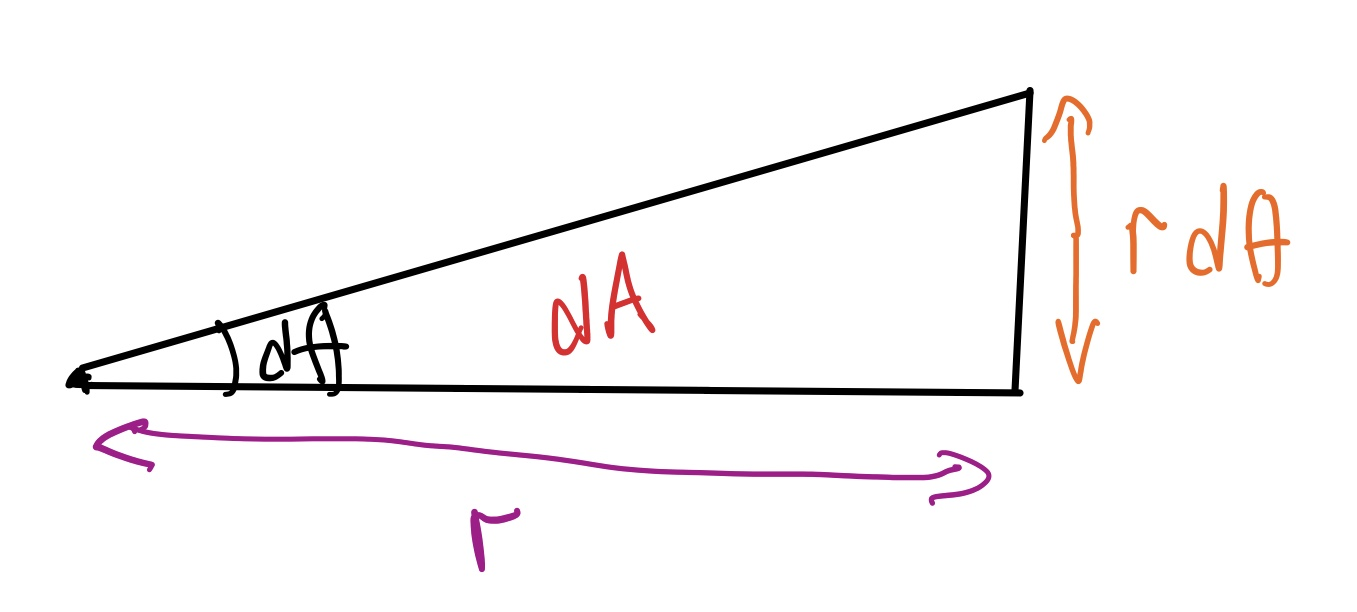
\includegraphics[width=80mm]{sketch.jpg}
	\caption{This square is the infinitesimal area dA that the planet has moved by a infinitesimal time interval dt}
	\label{fig:1bplot}
\end{figure}

Figure \ref{fig:1bplot} shows us that the area is:

\begin{equation}
    dA=\frac{1}{2}r^2d\theta
\label{eq:dA}
\end{equation}

We now want to find an infinitesimal area where the planet has moved around the sun, over an infinitesimal time step, where we use equation \ref{eq:dA}.

\begin{align}
    \frac{dA}{dt}&=\frac{1}2{r^2}\frac{d\theta}{dt}\\
    &=\frac{1}{2}rv_\theta
    \label{eq:dadt}
\end{align}
And the definition of angular momentum is given as
\begin{align}
    L=mrv_\theta
     \label{eq:L}
\end{align}

With equation \ref{eq:L} and \ref{eq:dadt} we can show that the angular momentum is conserved:
\begin{align*}
    \frac{dA}{dt}=\frac{1}{2}\frac{L}{m}
\end{align*}

Since $\frac{dA}{dt}$=constant and the mass m is constant it means that the angular momentum also is constant and therefore also conserved \cite{96}.  

\subsection{Testing forms of the force}

The force $F_g$ is on the form of an inverse square force. We can replace the r squared in \ref{eq:G} with a $\beta$ which we can alternate $\beta \in [2,3]$ . This gives us the equation:

\begin{align}
    \mathbf{F}_G=-\frac{GM_{\odot}M_{planet}}{r^{\beta}}\frac{\mathbf{r}}{r}
    \label{eq:F_b}
\end{align}

\subsection{Escape velocity}
We will now look at a planet which begins at a distance 1 AU from the sun, 
and see how fast the initial velocity must be for the planet to be able to escape the sun. We find the analytical solution to compare it to our numerical solution. The analytical expression is given by:

\begin{align}
    \mid{\mathbf{V}_{esc}}\mid=\sqrt{\frac{2GM_{\odot}}{r}}
    \label{fig:Vesca}
\end{align}

By plugging equation \ref{eq:G_M} into \ref{fig:Vesca}, and use that our initial position of the planet is $r=AU$ we get

\begin{align}
\mid{\mathbf{V}_{esc}^2}\mid&=\frac{2\cdot 4\pi^2AU^3}{yr^2}\cdot\frac{1}{r}\\
&=\frac{2\cdot 4\pi^2AU^3}{yr^2}\cdot\frac{1}{AU}\\
\mid{\mathbf{V}_{esc}}\mid&=2\sqrt{2}\pi\cdot\frac{AU}{yr}
\end{align}

\section{Appendix} % Her kommer appendix.
\subsection{Forward Euler}
The forward Euler method is an algorithm to estimate the solution of a differential equation. The Forward Euler method  finds the next positions $\mathbf{r}_{i+1}$ by using the position we are at $\mathbf{r}_{n}$, a small time step $dt$ and the derivative of its position. Which can be expressed as:

\begin{equation}
\mathbf{r}_{n+1}=\mathbf{r}_n + \mathbf{r}_n'\cdot dt
\label{eq:yn1}
\end{equation}

Where $\mathbf{r}_n'$ is the derived of the current position. This algorithm is an abbreviated version of a Taylor expansion, where we only expand the series one step at a time. By doing this we will get a local truncation error, which causes an error for each step we take:

\begin{equation}
\begin{split}
&\mathbf{r}(t_n+dt)=\mathbf{r}_{n+1}\\
=&\mathbf{r}(t_n)+dt\bigg(\mathbf{r}'(t_n) + \frac{\mathbf{r}''(t_n)}{2!}dt + ... + \frac{\mathbf{r}^p(t_n)}{p!}dt^{p-1}\bigg) \\
&+ O(dt^{p+1})
\end{split}
\label{eq:ytndt}
\end{equation} 

Where $O(dt^2)$ is the local truncation error. Since the Forward Euler method is a first-order method, the local truncation error will be proportional to the square of the step size.

In our case $\mathbf{r}(t_n) \rightarrow \mathbf{r}_n$ is the position, $\mathbf{r}'(t_n)=\mathbf{v}(t_n) \rightarrow \mathbf{r}'_n=\mathbf{v}_n$ is the velocity and $\mathbf{r}''(t_n)=\mathbf{a}(t_n,r_n) \rightarrow \mathbf{v}_n'=\mathbf{a}_n$ is the acceleration. The update of our position and velocity with a  time step is then given as  
\begin{align*}
    \mathbf{r}(t_{n+1})&=\mathbf{r}(t_n) + \mathbf{v}(t_n)dt + O(dt^2)\\
    \mathbf{r}_{n+1}&=r_{n} + v_{n}dt + O(dt^2)\\
    \mathbf{v}(t_{n+1})&=\mathbf{v}(t_n)+\mathbf{a}_ndt + O(dt^2)\\
    \mathbf{v}_{n+1}&=\mathbf{v}_n +\mathbf{a}_n dt + O(dt^2)
\end{align*}
Hence, the forward Euler algorithm will look like:
\begin{align*}
    \mathbf{r}_{n+1}&=\mathbf{r}_n+\mathbf{v}_ndt\\
    \mathbf{v}_{n+1}&=\mathbf{v}_n+\mathbf{a}_ndt\\
    t_{n+1}&=t_n + dt
\end{align*}

\subsection{Velocity Verlet method}
The Velocity Verlet method is based on the kinematic equations for a moving object, which in our case is a planets orbit around the sun. If we want to find the next time step for the velocity and position we do an approximation and use a Taylor-expansion:    

\begin{align*}
\mathbf{r}(t\pm dt)&=\mathbf{r}(t)\pm \mathbf{r}'(t)dt + \frac{\mathbf{r}''(t)}{2}dt\\ + O(dt^3)
\end{align*}

This gives us the position and velocity:

\begin{align}
    \mathbf{r}_{n+1}&=\mathbf{r_n}+\mathbf{v}_n dt + \frac{\mathbf{a}_n}{2}dt^2+O(dt^3)
    \label{eq:r_n+1}
    \end{align}
    \begin{align}
    \mathbf{v}_{n+1}&=\mathbf{v}_n+\mathbf{a}_ndt+\frac{\mathbf{v}''_n}{2}dt^2 + O(dt^3)
     \label{eq:v_n+1}
\end{align}

We need to define $\mathbf{v}''_n$. We do this by by defining the next step in acceleration $\mathbf{a}_{n+1}$:

\begin{align*}
    \mathbf{a}_{n+1}=\mathbf{v}'_{n+1}=\mathbf{v}'_n+\mathbf{v}''_ndt + ...
\end{align*}

We can rewrite this as:

\begin{align}
        \mathbf{v}''_n=\frac{\mathbf{v}'_{n+1}-\mathbf{v}_n'}{dt}
    =\frac{\mathbf{a}_{n+1}-\mathbf{a}_n}{dt}
    \label{eq:v_n}
\end{align}

By inserting equation \ref{eq:v_n} into equation \ref{eq:v_n+1} we get the general algorithm for the Velocity Verlet \cite{95}:

\begin{align*}
    \mathbf{r}_{n+1}&=\mathbf{r}_n+\mathbf{v}_ndt+\frac{\mathbf{a}_n}{2}dt^2+O(dt^2)\\
    \mathbf{v}_{n+1}&=\mathbf{v}_n+\frac{\mathbf{a}_{n+1}-\mathbf{a}_n}{2}dt+O(dt^3)
\end{align*}

\bibliography{References} % Kilder.
\begin{thebibliography}{9}
\bibitem{94}
	NASA, 2008, Orbits and Kepler's laws
\bibitem{95}
	Holm, C, 2013, Simulation Methods in Physics 1 
\bibitem{96}
	Hansen, F.K., 2019, Celestial Mechanics: calculating the orbits from AST2000
\bibitem{97}
	 Wikipedia, 2020, Tests of general relativity
\end{thebibliography}

\end{document}